%----------------------------------------------------------------------------------------
%	DOCUMENT CONFIGURATIONS
%----------------------------------------------------------------------------------------

\documentclass[]{article}

\usepackage{graphicx} % To include figures
\usepackage[utf8]{inputenc}
\usepackage{fancyhdr} % Required for custom headers
\usepackage{lastpage} % Required to determine the last page for the footer
\usepackage{extramarks} % Required for headers and footers
\usepackage[a4paper, top=4cm, bottom=4cm, left=3.3cm, right=3.2cm]{geometry}
%for the bibliography
\usepackage{booktabs}
\usepackage{url}
\usepackage{tocloft}

\renewcommand{\baselinestretch}{1.5}

% Set up the header and footer
\pagestyle{fancy}
\lhead{Carlos Pérez López} % Top left header
%\chead{\hmwkClass\ (\hmwkClassInstructor\ \hmwkClassTime): \hmwkTitle} % Top center header
\rhead{ASD Assignment: 3D Game} % Top right header
%\lfoot{\lastxmark} % Bottom left footer
%\cfoot{} % Bottom center footer
\rfoot{Page\ \thepage\ of\ \pageref{LastPage}} % Bottom right footer
\renewcommand\headrulewidth{0.4pt} % Size of the header rule
\renewcommand\footrulewidth{0.4pt} % Size of the footer rule


\title{
\vspace{2in}
\textmd{\textbf{ASD Assignment: 3D Game}}\\
\vspace{0.1in}
{\today}\\
\vspace{3in}
}

\author{\textbf{Carlos Pérez López}}
\date{}

\begin{document}

\maketitle % Insert the title, author and date

% If you wish to include an abstract, uncomment the lines below
% \begin{abstract}
% Abstract text
% \end{abstract}

\setlength\parindent{24pt} % Removes all indentation from paragraphs

\renewcommand{\labelenumi}{\alph{enumi}.} % Make numbering in the enumerate environment by letter rather than number (e.g. section 6)
\renewcommand{\cftsecleader}{\cftdotfill{\cftdotsep}}

\newpage
\tableofcontents
\newpage


%----------------------------------------------------------------------------------------
%	SECTION 1
%----------------------------------------------------------------------------------------

\section{Overview of the game}

This game was in first intance driven by a clear idea in the author's mind and the aim of introducing himself to computer graphics tecniques and concepts and game programming. As a matter of fact,
research in games is wide but shallow, and there are not strong standards established besides the ones inherited from computer applications development. Contrary to other disciplines of computer
graphics such as flocking systems, renderers, raytracers, crowd simulation, particles etc. the publications are not so solid and abundant. Game programming comprises a lot of different fields, and
the ability of integrating all of them properly and functionally is adquired primarily by experience.\\

The game named Rias Baixas is ambiented in a world of mafia and gangsters, where the player will have to transport an important package in a speed boat. The gameplay takes place on the sea, and the main
elements of the game are boats. Due to this, the behaviour of objects on fluids has a very important role in this project. Although it is not finished, the main functionallities are implemented and
so far it is presented a strong prototype that might become in a comercial game in the future.\\


Another sub-system of great importance in games, and in this particular one, is the AI. The player can find different objects with different behaviours on his path (so a way of relating objects and behaviours will
be needed) and, mainly, their purpose is slow down the advance of the speed boat. In this way, boats which crosses the sea can be found, or boats that are simply floating on it, or others with more complex behaviours. There is
a special object which is the Police Boat, and the player, in order to win, must reach the coast without being caught by it. In addition, a set of cameras is provided and the player might use the back
camera to check if some police boat is chasing him. Combining this elements, a simple but entertaining game prototype was built and in the future it might be finished and ported to other platforms.

 
%----------------------------------------------------------------------------------------
%	SECTION 2
%----------------------------------------------------------------------------------------

\section{Final Design}

After refactoring several times and trying different approaches from the initial design, this final one was achieved (see complete class diagram in \emph{/Diagrams}). The intention was to design
system where flexibility, decoupling, scalability and simplicity were the main key points. Therefore, several design patterns were used to create the class structure. To present the design in a tidy way, the different
parts or modules will be treated and discussed in each of the next paragraphs.

In order to model the different stages that a game can go through (menu, story, score, gameplay, etc) a state pattern was chosen. In this particular game, we count with three different states: \emph{GameMenu },
\emph{GameStory} and \emph{GamePlay} in which each method \emph{run} performs the process of the state and implements a state transition, as a pure state machine or automaton. See figure \ref{fig:stateDiagram}

\begin{figure}[!htb]
\begin{center}
\includegraphics[width=0.5\textwidth]{images/stateDiagram.eps}
\caption{State Diagram for the Game}
\label{fig:stateDiagram}
\end{center}
\end{figure}

The instances of the objects of the game world belong to the class \emph{Object}. It offers the state and behaviour needed for the simple objects which just differ in mesh and state information such as
\emph{MusselFarm} and \emph{FisherBoat} (But they differ in motion behaviour, which is unacoplated from this class; this is explained in the next paragraph). Other objects which need more specific features, such
as the \emph{SpeedBoat} or the \emph{PoliceBoat}, specialize the \emph{Object} class and refine certain methods. They way the communication happens between the world and the \emph{GamePlay} is using
an observer pattern. The \emph{GamePlay} (the observable) keeps a list with all the objects in the game world (the observers), and it notifies them when they need to update their internal state (such as position), 
which occurs once per iteration of the game loop. See figure \ref{fig:obsSeq} \\

\begin{figure}[!htb]
\begin{center}
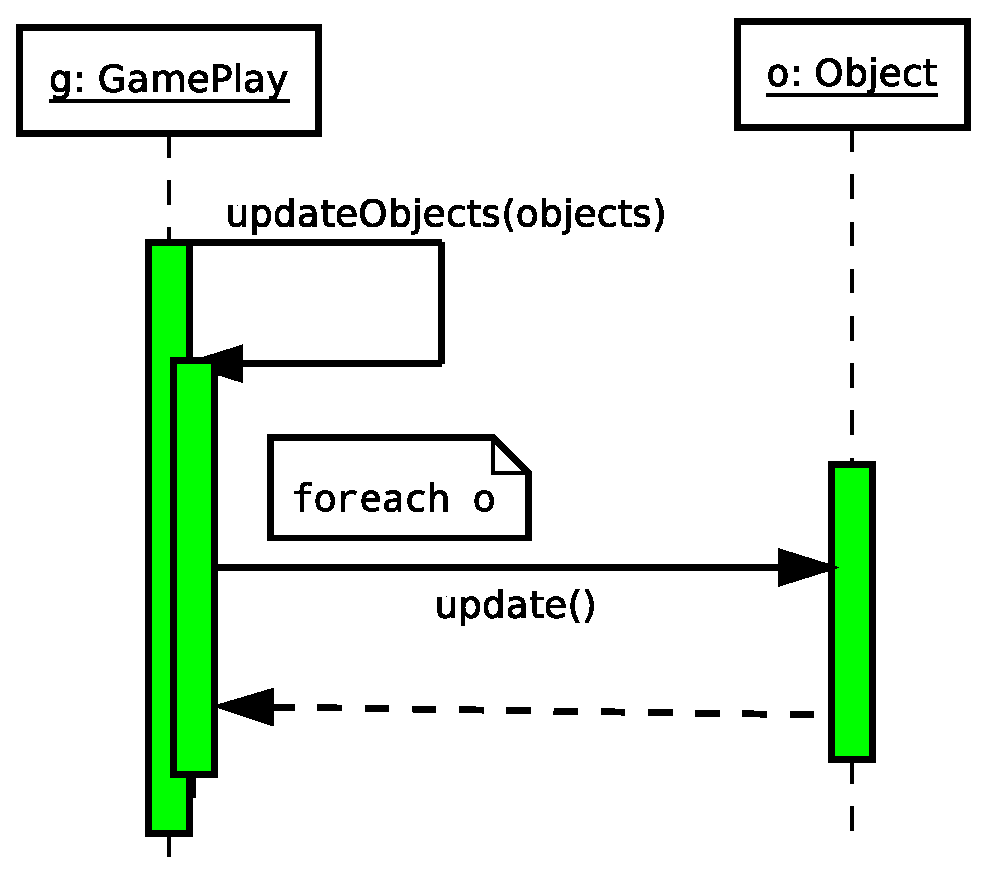
\includegraphics[width=0.5\textwidth]{images/observerSequence.eps}
\caption{Sequence Diagram for GamePlay-Objects}
\label{fig:obsSeq}
\end{center}
\end{figure}

The part of the system which conforms the AI resides on the class \emph{Behaviour} and its descendants. The base behaviour stores the full state that an entity needs to move around the world, since the mass, transformation
linear velocity, angular velocity, etc. till its degrees of freedom in the space. The basic motion is a very simple floating movement, which just oscilates up and down following a sinus function, and which all
the specific behaviours may use in their refined  movements. Each object stores an instance of a behaviour, which might be implemented for any of the set of the defined behaviours: \emph{Floating}, 
\emph{Horizontal}, \emph{Vertical} or \emph{Diagonal}. This is no more than a strategy pattern, where each object
is unware which specific behaviour has referenced, and it is extremely scalable because new behaviours can be added in next versions. In the figure \ref{fig:behaviours} the predefined behaviours are shown.\\

\begin{figure}[!htb]
\begin{center}
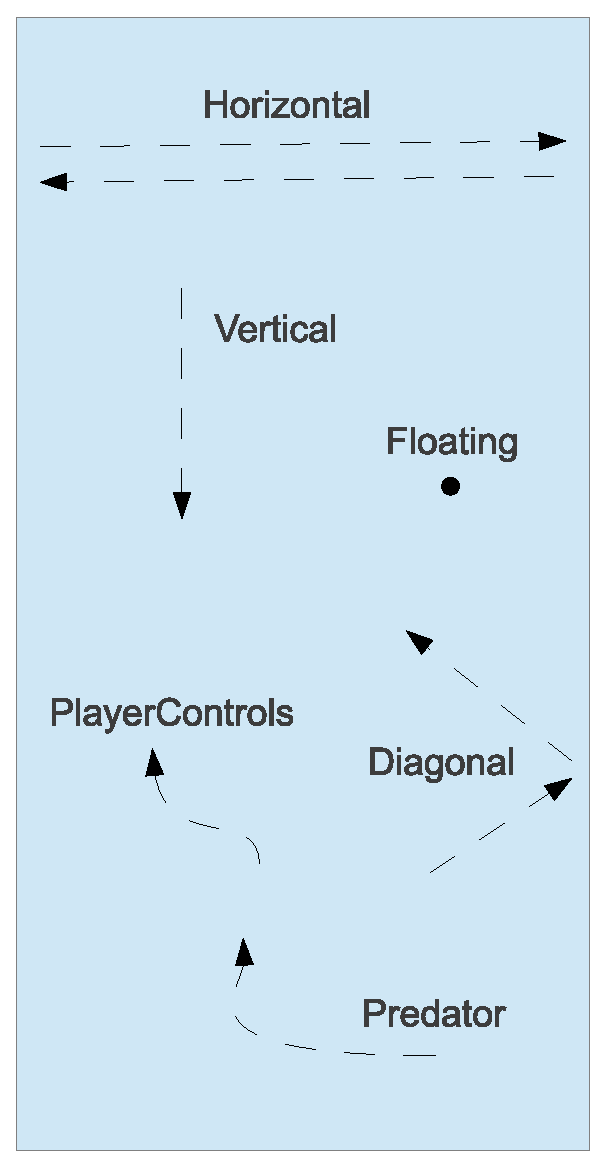
\includegraphics[width=0.25\textwidth]{images/behaviours.eps}
\caption{Different behaviours in the game}
\label{fig:behaviours}
\end{center}
\end{figure}

A special behaviour needs a little bit of attention. The \emph{PlayerControls} behaviour is the one which performs the user input, and it is updated from the GamePlay in the same way that a observer
(This will be explained in the speed boat section).
In the way this was designed, this class can also serve as a controller interface to other higher-level behaviours. The behaviour \emph{Predator} does this, and will be explained in the section of the police boat.
In the figure \ref{fig:straSeq} the complete sequence diagram is presented.\\

\begin{figure}[!htb]
\begin{center}
\includegraphics[width=0.8\textwidth]{images/strategySequence.eps}
\caption{Sequence Diagram for GamePlay-Objects-Behaviour}
\label{fig:straSeq}
\end{center}
\end{figure}

It is also worthy to mention the class where all the graphics and drawing functionalities are encapsulated, the \emph{Renderer} class. In the most upper level, the \emph{Game} stores a refence of
the Renderer selected to draw our world (in this case, the one buil-in with the system), and this is passed to each state of the game in order to render using the same graphic context. \\

These are the elements which make this design robust. Then, there are other important classes such as the \emph{PhysicsEngine} and the \emph{Parser}, that comprise a series of decisive methods. But
in terms of design, they are structured as simple inheritance, which is still highly flexible if we consider the power of polimorphysm.


%----------------------------------------------------------------------------------------
%	SECTION 3
%----------------------------------------------------------------------------------------

\section{The Speed Boat}

The speed boat is the main character of the game. It stores a reference of a \emph{PlayerControls} behaviour, which is updated every iteration of the loop by the user input. This behaviour allows
to the user advance in a track of the sea: moving left, right and accelerating; and all these movements are permorfed following how a real boat would do them, respecting the rules of physics and
inertias and combering.\\

This speed boat, according to the background story, is transportating a high valuable load and the user has to avoid to miss it. In the \emph{Collision Event} (this type of event will be explained in the last section)
the object of type speed boat reduces its load, depending on which other object the user collides with (this feature is not implemented yet). Therefore, if the load reaches 0, the user would lose
and the game would be over. On the other hand, if the user can reach the end of the track (the coast) with some batch he would win, but his score might depend on the amount.


%----------------------------------------------------------------------------------------
%	SECTION 4
%----------------------------------------------------------------------------------------

\section{The Police Boat}

The police boat uses a specific behaviour which differs a bit from the others. In this case, \emph{Predator} uses \emph{PlayerControls} as a controller interface to move the object, and it only
implements the chasing algorithm. \\

The class \emph{Predator} keeps a reference to the object which it pursuits, the prey, and execute movements according with its position. So far a very simple algorithm is implemented but, in the future, 
it might be added more advanced pathfinding algorithms such as A star.

%----------------------------------------------------------------------------------------
%	SECTION 5
%----------------------------------------------------------------------------------------

\section{Algorithm for the Collision Detection}

The specific physiscs engine built-in with this project implements a basic collision detection based on bouncing espheres, \emph{BEPhysicsEngine}. But it is not so simple, since the struct \emph{degreesOfFreedom} 
needs to be calculated. This data has a critical function due to it is used by the AI in order to take decisions about the direction of the movements.\\

The degrees of freedom of an object are these: up, down, forward, backward, left and right and their computation is performed based on projections. Let us have the example of two colliding 
  objects and let us analyze the top projection. If we viewed the scene from the top, we could build a 2D coordinate system where the centers of the objects would have certain
  x1, y1 and x2, y2. Employing the relations between the x variables and the slope of the line traced from O1 to O2 it can be determined the side in which the collision takes place. In our
  specific example (see \ref{fig:dof}) we notice that $x2 > x1$ and $slope > 1$, thus the degrees of freedom of our objects change in this way: $O1.dof.forward = false$ and $O2.dof.backward = false$; what means 
  that the AI cannot steer them in those directions.

\begin{figure}[!htb]
\begin{center}
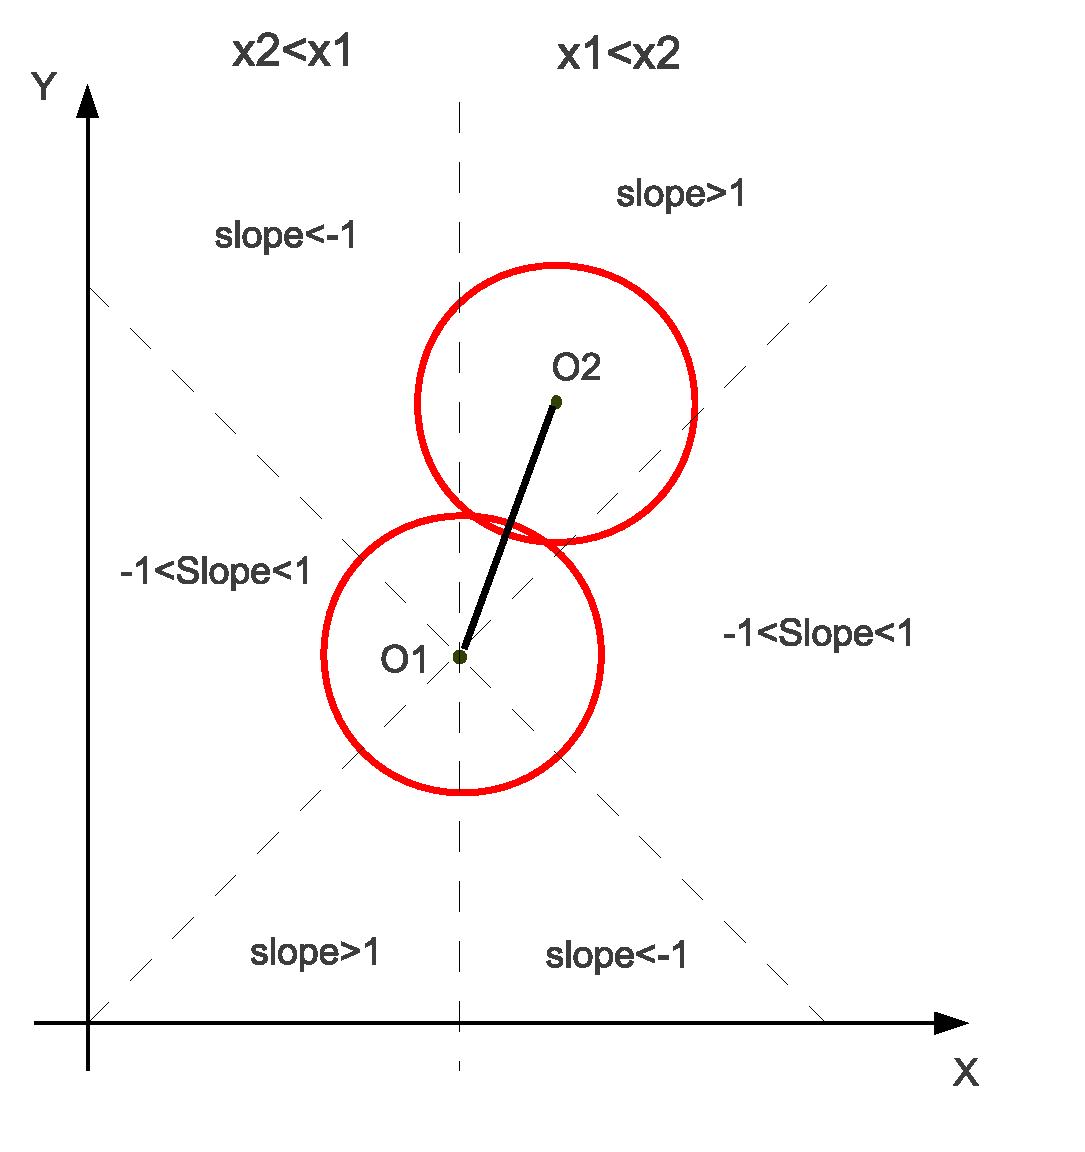
\includegraphics[width=0.5\textwidth]{images/dofCalculation.eps}
\caption{Top projection of a collision}
\label{fig:dof}
\end{center}
\end{figure}



%----------------------------------------------------------------------------------------
%	SECTION 5
%----------------------------------------------------------------------------------------

\section{Collision Events}

The collisions events system works as a sort of observer again. When the physics engine checks that a collision takes place, it triggers the corresponding \emph{collisionEvent} from both colliding objects.
This mechanism is very important, thus allows to objects change their state or perform any action due to a collision.\\

This method, member of the class \emph{Object}, recieves as argument the obect against the collision happens and, therefore, it can send messages and ask for services to it. This is very useful to identify situations
like when the police boat finally catches the speed boat or the collisions which can reduce the load of the speed boat.\\

In addition, these collisions events were thought like this from the beginning to also allow the possibility of rising radio conversations with gags when they occur.


\end{document}
